\documentclass[10pt, a4paper]{article}
\usepackage[utf8]{inputenc}
\usepackage[spanish]{babel}
\usepackage[margin=1.5cm]{geometry}
\usepackage{graphicx}
\usepackage{booktabs}
\usepackage{hyperref}
\hypersetup{
	colorlinks=true,
	citecolor=black,
	linkcolor=black
}
\usepackage{cleveref}
\usepackage{enumitem}
\usepackage{etoolbox}
\usepackage{authblk}
\usepackage{xcolor}
\usepackage{float}
\usepackage{caption}
\usepackage{subcaption}
\captionsetup{font=small}

\makeatletter
\apptocmd{\@floatboxreset}{\centering}{}{}
\makeatother

\title{\Large \textbf{Proyecto Sistemas Distribuidos: informe de la segunda entrega}}
\author[1]{Solon Losada Cadena}
\author[1]{Juan Pablo Peña Bernal}
\author[1]{Alejandro González Ochoa}
\affil[1]{Departamento de Ingeniería de Sistemas, Pontificia Universidad Javeriana, Bogotá, 110231, Colombia.}
\date{}

\begin{document}

	\maketitle
	\vspace{-1.2cm}

	\begin{center}
		\small Autores: \href{mailto:solon.losadac@javeriana.edu.co}{\color{blue}solon.losadac@javeriana.edu.co}; \href{mailto:jp.penab@javeriana.edu.co}{\color{blue}jp.penab@javeriana.edu.co}; \href{mailto:alejandro.gonzalez.o1055@javeriana.edu.co}{\color{blue}alejandro.gonzalez.o1055@javeriana.edu.co}
	\end{center}

	\begin{center}
		\textbf{Docente:} Ricardo Hjalmar González García \\
		\textbf{Fecha:} 22 de noviembre de 2026 \\
		\textbf{Video:} \href{https://drive.google.com/drive/folders/1UDNqkXTleU3nn4BU5am9ttJe5K5cbXOO?usp=sharing}{\color{blue}enlace al video de la segunda entrega}
	\end{center}

	\vspace{0.4cm}

	% ---------------------------------------------------------
	% SEGUNDA ENTREGA (Max 5 pages)
	% ---------------------------------------------------------

	{\small \textbf{\textit{Keywords}---}Sistema de Reserva de Boletos, ZeroMQ, escalabilidad, tolerancia a fallos, pruebas de rendimiento.\par}

	\section{Objetivo y entorno de medición}
	\label{sec:entorno}

	Comparamos la arquitectura base del SRB (un proceso de cada tipo, como en la figura del enunciado) con la arquitectura escalable de esta entrega. Con 3, 5 y 8 clientes simultáneos medimos la media y la desviación estándar del tiempo de respuesta de consulta y de reserva, y las transacciones por minuto (TPM) de cada una. \textbf{Todos los procesos corrieron en una sola máquina}, no en las tres del despliegue: las mediciones no incluyen latencia de red y las cifras absolutas no son comparables con las de un despliegue distribuido, pero las dos arquitecturas se midieron en las mismas condiciones y entre sí sí se comparan.

	\begin{table}[H]
		\centering\small
		\begin{minipage}[t]{0.56\textwidth}
			\centering
			\begin{tabular}{@{}lp{0.68\linewidth}@{}}
				\toprule
				CPU & AMD Ryzen 7 5700U (8 núcleos, 16 hilos) \\
				RAM & 14 GiB \\
				SO & Linux 7.3 (CachyOS) \\
				Software & Python 3.14, pyzmq 27.3 (libzmq 4.3.5), SQLAlchemy 2.0, psycopg 3 \\
				Base de datos & PostgreSQL 16 en Docker, misma máquina \\
				Medición & \texttt{scripts/benchmark.py}, un CSV por cliente, \texttt{statistics} de Python \\
				\bottomrule
			\end{tabular}
		\end{minipage}\hfill
		\begin{minipage}[t]{0.40\textwidth}
			\centering
			\begin{tabular}{@{}lcc@{}}
				\toprule
				Componente & Base & Escalable \\
				\midrule
				GT & 1 & 1 \\
				RMC & 1 & 4 \\
				Cancelación & 1 & 2 \\
				Hilos de persistencia & 1 & 8 \\
				\bottomrule
			\end{tabular}
		\end{minipage}
		\caption{Hardware y software de las mediciones (izquierda) y configuración de cada arquitectura (derecha).}
		\label{tab:entorno}
	\end{table}

	Las réplicas del RMC y de cancelación se conectan al gestor de transacciones (GT), que reparte el trabajo por turnos con ROUTER/DEALER y PUSH/PULL, de modo que añadirlas no exigió cambiar el GT ni los clientes. En ambas arquitecturas un supervisor lanza los procesos de la capa de servicios y relanza el que se detenga.

	\section{Metodología}
	\label{sec:metodo}

	Cambiamos Locust, la herramienta prevista en la primera entrega, por un generador de carga propio en Python, porque su adaptador para ZeroMQ no cabía en el plazo. Cada cliente es un proceso que guarda en un CSV el tiempo de cada operación, y de ahí salen la media, la desviación y los TPM. Los escenarios siguen el enunciado: con 3 clientes, 2 solo consultan y 1 consulta y reserva; con 5, 3 solo consultan y 2 reservan y modifican; con 8, 4 solo consultan y 4 reservan y modifican. Cada corrida dura 120 s y antes de cada una se recrea la base con 50 eventos, 20 de ellos con dos ocurrencias.

	A 20 solicitudes por minuto por cliente, el mínimo del enunciado, ningún componente se acerca a su límite y ambas arquitecturas darían lo mismo. Por eso cada cliente se configuró a 6\,000 solicitudes por minuto: ninguno llega a ese valor, porque envía la siguiente solicitud apenas recibe la respuesta (ciclo cerrado) y el sistema trabaja a su capacidad máxima. Por la misma razón usamos 100\,000 asientos por ocurrencia en vez de 100, para que los rechazos por falta de cupo no distorsionaran la comparación. El tiempo de respuesta es el que mide el cliente entre enviar y recibir; los TPM son las operaciones completadas sin error técnico entre los minutos de la corrida, y el número de reservas en la base coincide con las exitosas que contaron los clientes.

	\section{Resultados}
	\label{sec:resultados}

	\begin{table}[H]
		\centering\small
		\begin{tabular}{@{}rlrrrrr@{}}
\toprule
Clientes & Arquitectura & Consulta (ms) & Reserva (ms) & TPM consulta & TPM reserva & Errores \\
\midrule
3 & Base & 5.5 $\pm$ 3.1 & 8.5 $\pm$ 2.8 & 14\,488 & 2\,851 & 0 \\
3 & Escalable & 4.2 $\pm$ 1.1 & 8.7 $\pm$ 1.7 & 14\,810 & 2\,910 & 0 \\
\midrule
5 & Base & 17.4 $\pm$ 3.1 & 17.8 $\pm$ 3.0 & 10\,316 & 3\,459 & 0 \\
5 & Escalable & 5.5 $\pm$ 2.5 & 11.1 $\pm$ 3.0 & 17\,543 & 5\,287 & 0 \\
\midrule
8 & Base & 31.4 $\pm$ 4.5 & 31.7 $\pm$ 4.5 & 7\,636 & 3\,862 & 0 \\
8 & Escalable & 13.5 $\pm$ 7.8 & 20.7 $\pm$ 7.1 & 16\,026 & 6\,053 & 0 \\
\bottomrule
\end{tabular}

		\caption{Tiempo medio $\pm$ desviación estándar (ms), TPM de cada operación y errores técnicos por escenario.}
		\label{tab:resultados}
	\end{table}

	\begin{figure}[H]
		\centering
		\begin{subfigure}{0.49\textwidth}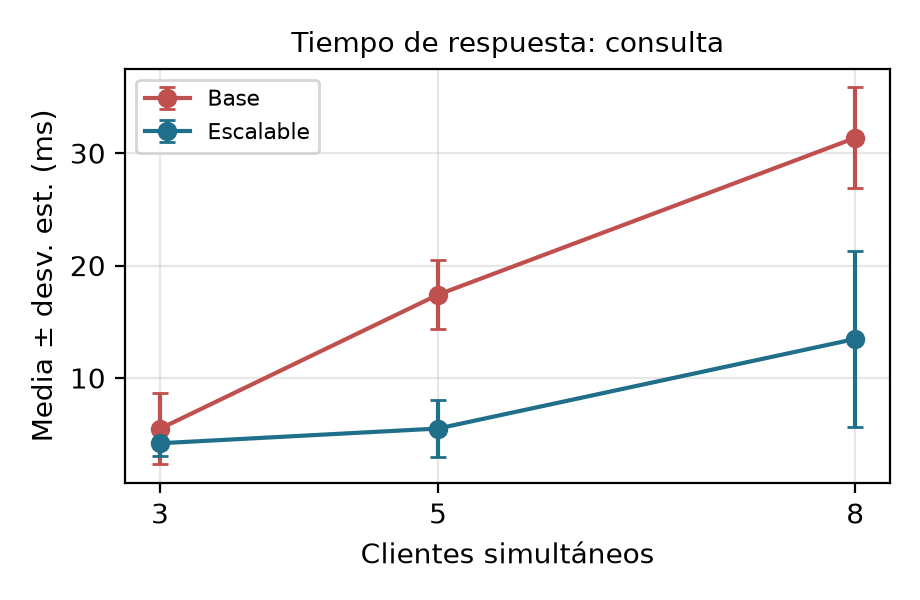
\includegraphics[width=\textwidth]{Images/rend_consulta_ms.png}\end{subfigure}
		\begin{subfigure}{0.49\textwidth}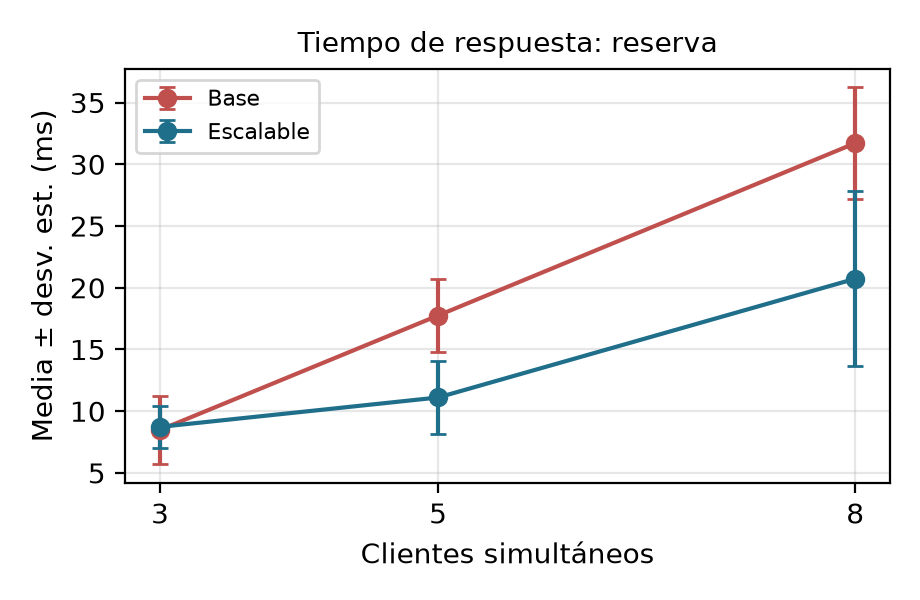
\includegraphics[width=\textwidth]{Images/rend_reserva_ms.png}\end{subfigure}
		\begin{subfigure}{0.49\textwidth}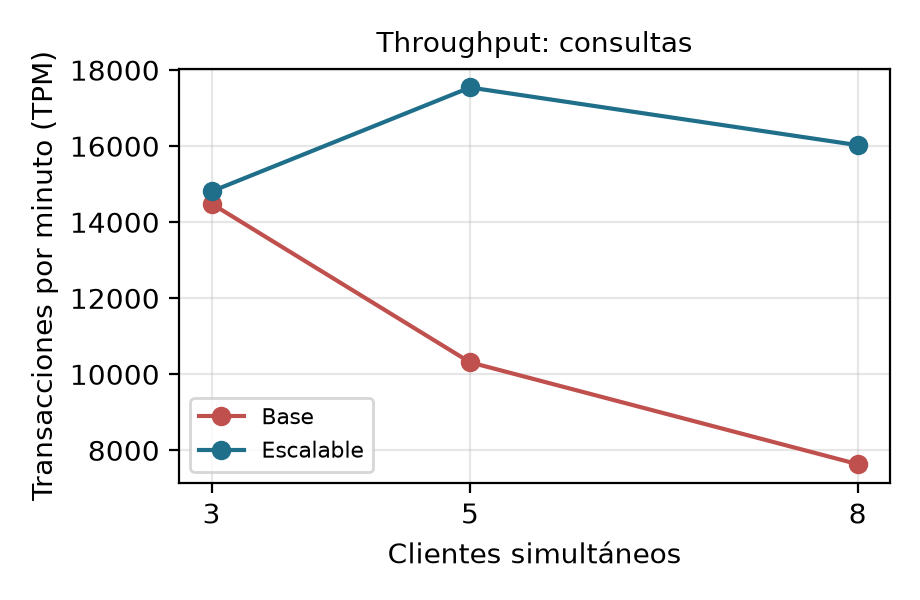
\includegraphics[width=\textwidth]{Images/rend_consulta_tpm.png}\end{subfigure}
		\begin{subfigure}{0.49\textwidth}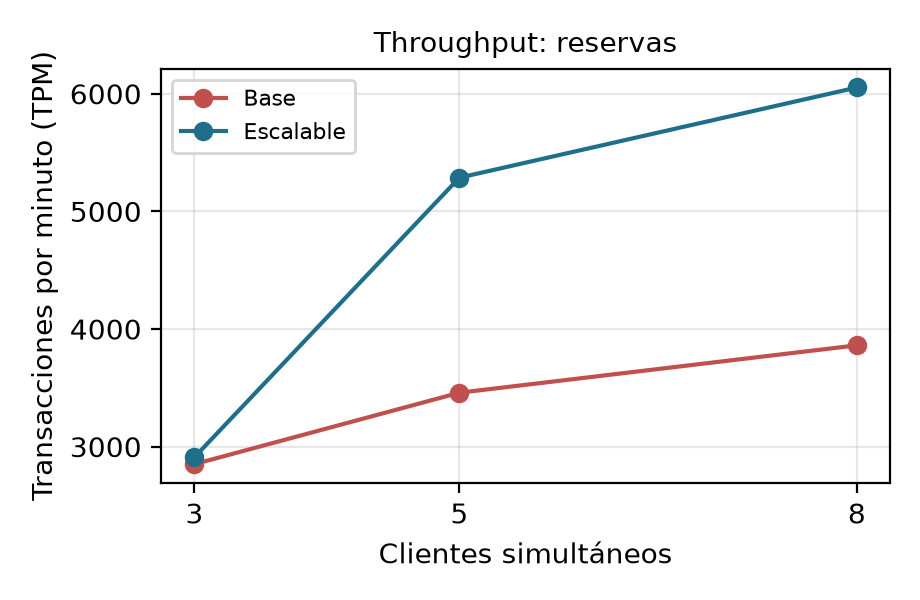
\includegraphics[width=\textwidth]{Images/rend_reserva_tpm.png}\end{subfigure}
		\caption{Tiempo de respuesta (arriba, media con barras de desviación estándar) y TPM (abajo) frente al número de clientes.}
		\label{fig:graficas}
	\end{figure}

	\section{Análisis}
	\label{sec:analisis}

	Con 3 clientes no hay diferencia apreciable. Solo uno reserva y un RMC con un hilo de persistencia lo atiende sin cola: la reserva tarda 8.5 ms en la base y 8.7 ms en la escalable, y los TPM difieren 2\,\%, dentro del ruido. La consulta pasa de 5.5 a 4.2 ms, pero con desviaciones de 3.1 y 1.1 ms no podemos atribuirlo a la arquitectura.

	Con 5 y 8 clientes la base se satura. Su tiempo de respuesta crece casi en proporción al número de clientes (la consulta pasa de 5.5 ms con 3 clientes a 17.4 con 5 y a 31.4 con 8, y la reserva de 8.5 a 17.8 y a 31.7) y los TPM de consulta bajan de 14\,488 a 7\,636 aunque haya más clientes pidiendo. Es lo esperable de un sistema de capacidad fija que recibe más solicitudes de las que procesa. No medimos en qué componente se forma la cola; sospechamos del RMC y del hilo único de persistencia, que son lo que cambia entre arquitecturas.

	La arquitectura escalable absorbe esa carga. Con 5 clientes el tiempo de consulta baja 68\,\% y el de reserva 38\,\%, y los TPM suben 70\,\% y 53\,\%. Con 8 clientes la consulta baja 57\,\% y la reserva 35\,\%; los TPM de consulta se multiplican por 2.1 y los de reserva por 1.6. Ninguna de las seis corridas tuvo errores técnicos. La mejora es menor que el número de réplicas (cuatro RMC no dan cuatro veces más rendimiento) y las reservas mejoran menos que las consultas. No lo medimos, pero tres cosas lo explicarían: todas las solicitudes siguen pasando por un único GT, una reserva hace dos consultas y una escritura sobre una sola base PostgreSQL que serializa las escrituras sobre la misma fila, y clientes, servicios y base compartieron los núcleos de una máquina.

	También repetimos la corrida escalable de 8 clientes con la réplica de PostgreSQL en streaming activa. Las consultas de eventos se leyeron de ella, y primario y réplica terminaron con las mismas 12\,146 reservas y 1.4 ms de retraso. Los resultados fueron equivalentes (consulta 13.4 $\pm$ 7.8 ms y 16\,045 TPM; reserva 20.8 $\pm$ 7.1 ms y 6\,061 TPM): una lectura tarda cerca de 1 ms de los 13 ms de una consulta, y base y réplica comparten núcleos. La réplica da una copia de los datos y permite seguir respondiendo consultas si cae el primario, pero no más velocidad. Las reservas, modificaciones, cancelaciones y la comprobación de cupo van siempre al primario, así que no puede causar sobreventa.

	Para la tolerancia a fallos, \texttt{scripts/demo\_fallos.py} envía 24 reservas seguidas y, a mitad de camino, detiene con \texttt{kill -9} el GT (dos veces) y un RMC. El supervisor relanzó cada proceso, el cliente reintentó con el mismo identificador de petición y las 24 reservas quedaron guardadas una sola vez. Las operaciones afectadas tardaron unos 2.5 s (el tiempo de espera del cliente antes de reintentar) frente a unos 20 ms habituales: ese es el costo de la recuperación transparente.

	Respondiendo la pregunta del enunciado, el diseño escalable mejora las métricas solo cuando el sistema está saturado: con 5 y 8 clientes reduce el tiempo de consulta entre 57\,\% y 68\,\% y el de reserva entre 35\,\% y 38\,\%, y aumenta los TPM de consulta entre 70\,\% y 110\,\% y los de reserva entre 53\,\% y 57\,\%. Con 3 clientes no mejora.

	\section{Limitaciones}
	\label{sec:limites}

	Todo corrió en una máquina, con clientes, servicios y PostgreSQL compitiendo por la misma CPU; en tres máquinas la red añade latencia y las capas no comparten recursos. Cada configuración se midió una vez, sin intervalos de confianza, y la réplica solo en una corrida adicional, sin probarla con la base y la réplica en máquinas distintas. Con 20 solicitudes por minuto por cliente esperamos tiempos equivalentes en ambas arquitecturas.

\end{document}
